% what is shown in the GUI
% what is the difference between the two subject groups
% what is the objective for the subject
% what information is saved
% what is the assumed learning goal for the test group

\section{User training} \label{sec:M:usertraining}
This section provides information on how the visual feedback was presented to the subjects in the to experiment groups during the user training, and what the objective for the subjects was. \\
The user training interface contained the following feedback: an illustration of the movement needed to be performed, a horizontal bar visualizing the contraction level and a vertical bar plot visualizing which movement is being recognized by the control system, as shown in \figref{fig:feedbackGUI}. The difference in feedback given between subject group, lied in the information given in the vertical recognition bar plot.

\begin{figure}[H] 
\centering
	\subfigure[Test group user training interface.]
		{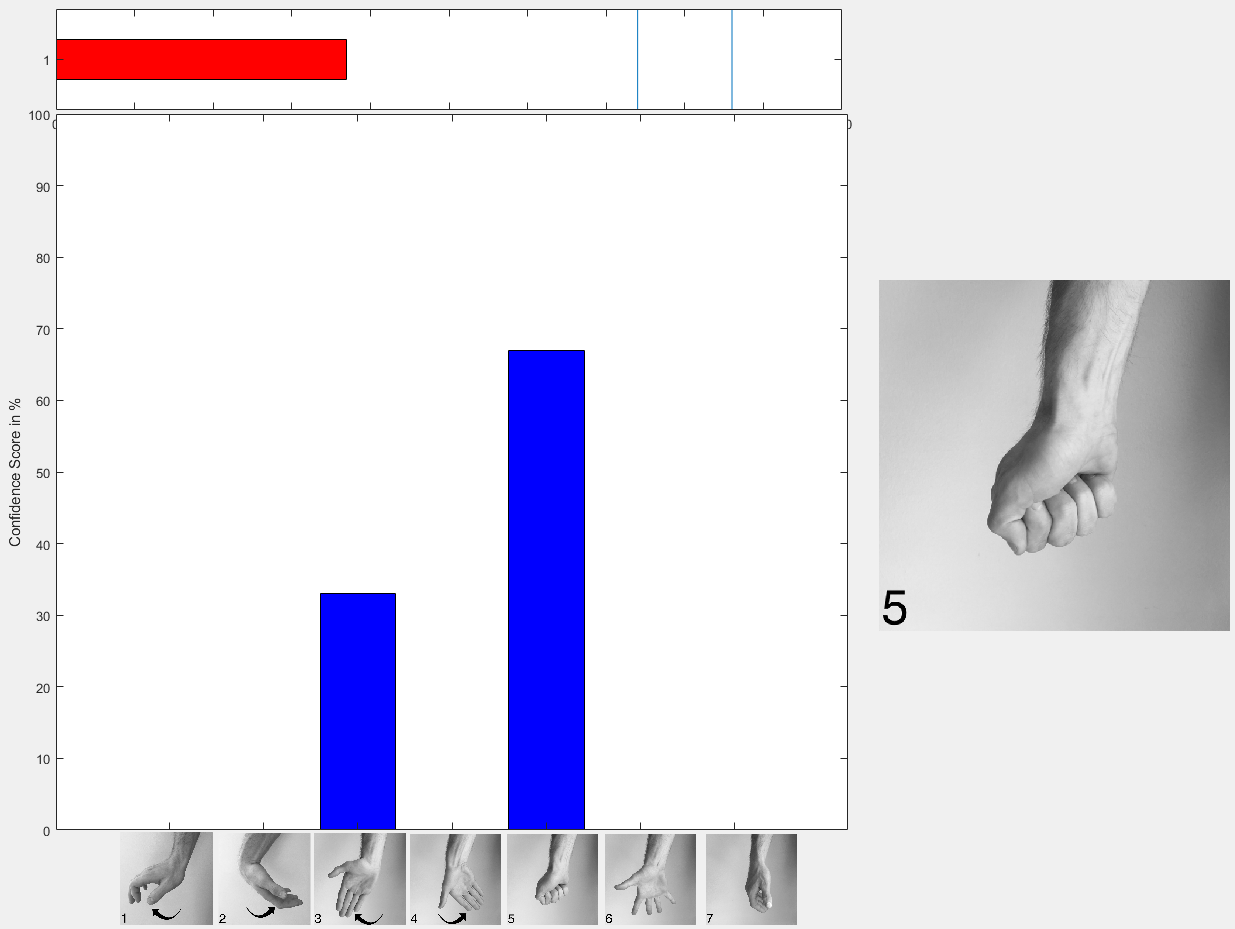
\includegraphics[width=.49\textwidth]{figures/xBackground/usertraintestGUI}}
	\subfigure[Control group user training interface.]
	    {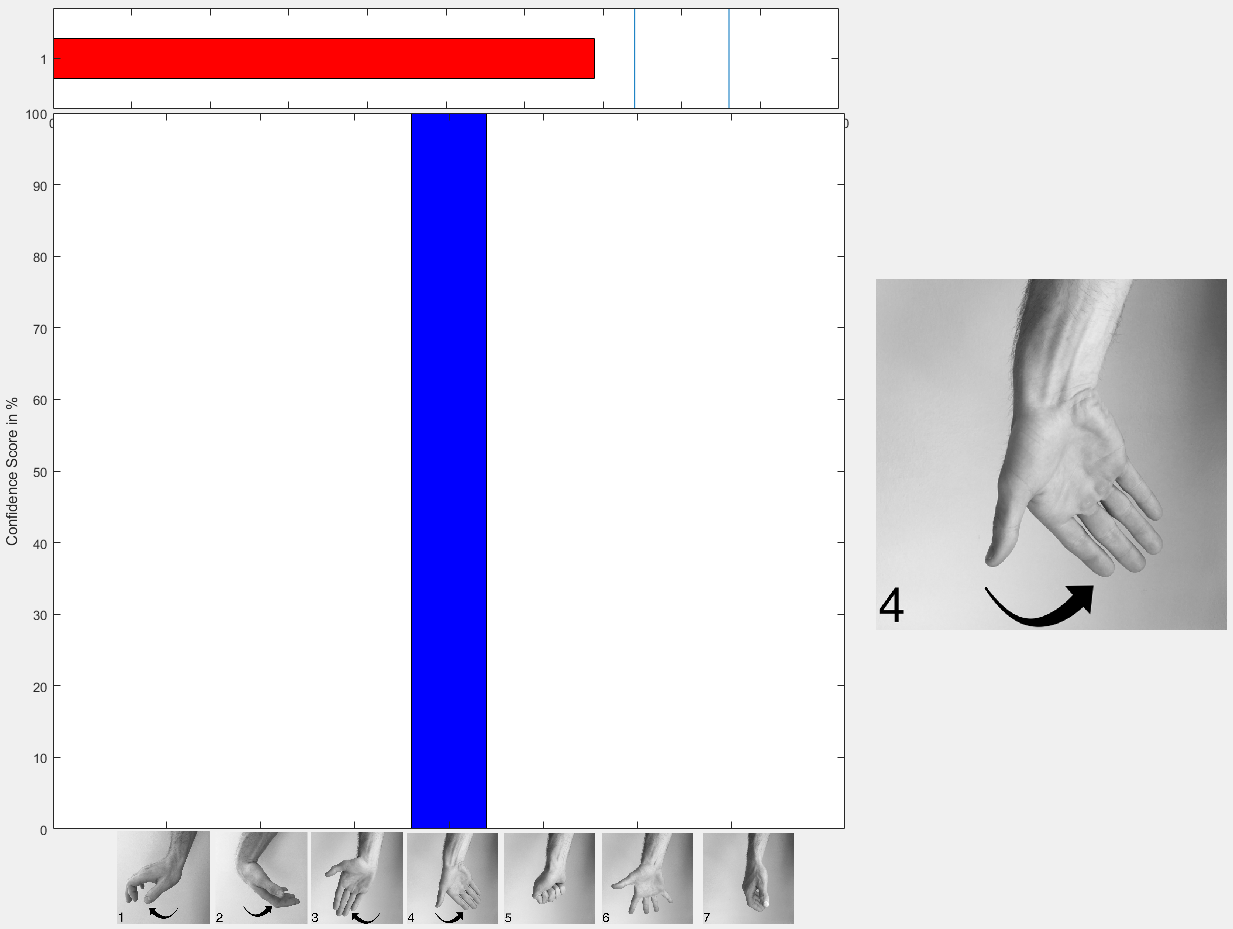
\includegraphics[width=.49\textwidth]{figures/xBackground/usertraincontrolGUI}}  
	\caption{Illustration of the user training interface for the test group (a) and the control group (b). The vertical bar plot indicates which movement is being recognized and the horizontal bar plot indicates contraction level. The two vertical lines in the contraction level bar plot illustrates the contraction level interval the subject must reach. The large picture of a movement indicates which movement needs to be performed. The difference between the feedback the two subject groups receive is the information given in the vertical recognition bar plot. The control group only sees a full bar of the movement the control system recognizes the most, whereas the test groups receives the exact recognition probabilities of all movements.}
    \label{fig:feedbackGUI}
\end{figure}

The illustration of the movement needed to be performed was shown for 30 seconds, after which an illustration indicating rest was shown for 7 seconds followed by a countdown from 3 to 1 seconds indicating the time left of the resting period. Thus, the subject needed to perform a movement for 30 seconds and rest for 10 seconds before another movement needs to be performed. The subjects needed to perform all movements in four different contraction level intervals of their maximal intensity, starting with the highest interval: 75-85~\%, 55-65~\%, 35-45~\% and 15-25~\%, visualized by the two vertical lines in the horizontal contraction level bar plot. The subjects needed to perform all movements in the same contraction level interval before moving to a new interval. The instructed movements were trained in a random order. \\
The horizontal bar showed the contraction level. This was calculated as the mean of the latest three intensity outputs as computed in \secref{sub:M:regression}, regardless of the movement being recognized. This resulted in a 400 ms delay in the visualization of the horizontal bar at the initiation of the training of a movement, due to the windowing used in feature extraction as mentioned in \secref{sub:M:featureExtraction}. However, the delay was not noticeable and the averaging of the intensity output resulted in a smooth visualization of the vertical bar. \\
The vertical bar plot showed which movement(s) the control system recognized. For a movement to be recognized as an active movement, the subjects had to perform the movement with more than 15~\% contraction intensity. The test group received information on the exact probabilities for the movements that were recognized. Thus, more bars could appear at the same time as seen in \figref{fig:feedbackGUI} (a). The purpose of this feedback was for the subjects to adapt to how the control system recognized the instructed movement. It gave the subjects the possibility of noting which movements that also were recognized when performing the instructed movement. When the instructed movement was not recognized with a 100 ~\% certainty the subject could use the information to slightly correct the performed movement until the control system recognized the instructed movement with a 100~\% certainty. This bar plot was calculated as the mean of the recognition certainties calculated from the latest three feature inputs, which resulted in a smooth visualization of certainties for the movements in the bar plot. \\
The control group only received information on which movement was recognized the most, represented as a single full bar at the recognized movement as seen in \figref{fig:feedbackGUI} (b). Thus, the control group was not informed on the exact probabilities of which movements the control system recognized. This bar plot was calculated as the movement with the highest certainty out of the mean of the recognition certainties calculated from the latest three feature inputs. \\
To motivate the subjects and to train the transition to and from resting position a task was included in the user training. The subjects were instructed in performing the instructed movement with a 100 \% certainty inside the instructed contraction level interval. When this was reached the horizontal bar would turn from red to green. The subjects were instructed in withholding the green colour for one second, after which the horizontal bar would turn blue and a light sound was played. After this task was reached the subjects was instructed in returning to rest and perform the task again. The objective for the subject was then to make the horizontal bar blue as many times as possible during an instructed movement of an instructed contraction level. The number of times the horizontal bar got blue during an instructed movement in an instructed contraction level was saved for later data analysis. \\

To summarize, the overall objective for the subjects during the user training was to adapt to how the control system recognized the performed movement. The user training was implement for the subjects to possibly improve their ability to use the control system. Their ability to use the control system was then evaluated in the modified Fitts' Law task. 











 







